%use in documents with \subfile{tex/intro}
\documentclass[../../master.tex]{subfiles}

\begin{document}

\section{RNA Secondary Structures}
\label{sec:theory:rna_secstructures}

	
%\todo{briefly establish RNA sequences and structures as an example of genotype-phenotype maps, and fitness landscapes. Might fit better into intro though, right after biological context?}
%\todo{\parencite{stadler_genotype-phenotype_2006, fontana_continuity_1998, ancel_plasticity_2000}}


%\todo{Don't like this segue} Now that it has been established what the structure hierarchy of RNA is, the focus will be shifted to secondary structure since that particular level of description is central to this work.

%\parencite{lorenz_viennarna_2011, lorenz_rna_2014}

In the literature, formal definitions of RNA secondary structure to be used in the context of combinatorial bioinformatics are usually quite similar.
They may differ in details like allowed base pairs or the number of allowed pairings \parencite{zuker_rna_1984}.
Here, a set of common rules is used to define legal pairings.
Additionally, an RNA secondary structure is viewed here as a set of base pairs, although other mathematical objects could be used instead, for example vertex-labelled graphs \parencite{hofacker_combinatorics_1998}.

An RNA sequence, i.e. the primary structure, can be viewed as as a word consisting of letters from the alphabet $\{\mathrm{A},\mathrm{C},\mathrm{G},\mathrm{U}\}$ representing the four RNA nucleotides.
Therefore, given a RNA sequence $r$ of length $N$, i.e. $r \in \{\mathrm{A},\mathrm{C},\mathrm{G},\mathrm{U}\}^N$, a  secondary structure of $r$ is a set of ordered pairs 
$(i, j)$ with $i < j$, where $i$ and $j$ denote paired positions satisfying the following rules \parencite{hofacker_rna_2005, hofacker_rna_2006}:
\begin{enumerate}[label=(\roman*), leftmargin=*, itemsep=0.4ex, before={\everymath{\displaystyle}}]
	\item for any two pairs $(i, j)$, $(k, l)$ with $i \leq k$: $i=k \Leftrightarrow j=l$ \label{eq:rule1}
	\item for any pair $(i, j)$: $j - i > 3$\label{eq:rule2}
	\item for any two pairs $(i, j)$, $(k, l)$ with $i \leq k$: $k<j \Rightarrow i<k<l<j$ \label{eq:rule3}
	\item for any pair $(i, j)$: $r_i r_j \in \{\mathrm{AU}, \mathrm{UA}, \mathrm{CG}, \mathrm{GC}, \mathrm{GU}, \mathrm{UG}\}$ \label{eq:rule4}
\end{enumerate}
The advantage of formulating rules like this lies in the straightforward way to implement them in computational methods.
Albeit seeming a bit convoluted, the intuition behind these rules is not too complex:

The first rule \ref{eq:rule1} specifies that each position participates in at most one base pair.
Rule \ref{eq:rule2} encompasses a simple steric constraint of RNA molecules; nucleobases too close to each other cannot form hydrogen bonds.
Rule \ref{eq:rule3} prohibits base pairs from crossing other base pairs in the same structure.
Finally, \ref{eq:rule4} provides some convenience, since restricting the allowed base pair identities to the most stable pairings reduces computational cost in stability-maximizing algorithms~\parencite{zuker_rna_1984, flamm_rna_1999} aside from distinguishing from tertiary structures.
A sequence and a structure are called compatible if they fulfill rule \ref{eq:rule4}.
This notion is often not imposed in defitions of secondary structure \parencite{hofacker_combinatorics_1998}, but it will be used later in \autoref{par:methods:seqspace}.

The terms \emph{noncrossing} or \emph{nested} structures are used synonymously for secondary structures characterized by these rules throughout this work.
\autoref{fig:strucrepresentation:a} depicts a secondary structure as a vertex-labelled graph representing a coarse-grained view of the polymer. 

%Depending on the formal framework used to describe RNA secondary structures, a multitude of visual representations of secondary structures exists.
%\todo{there are loads. some more interesting depending on mathematical framework (see reidys , tableaux, motzki paths and tangled diagrams)??}
%\todo{Later, I'll use some trees. maybe should introduce here}
%Here, the usage of basic visual representations is considered well fitting and relates directly to the definition using list of pairs.

\begin{figure}[!ht]
	\centering
	\begin{subfigure}[t]{0.5\textwidth}
		\centering
		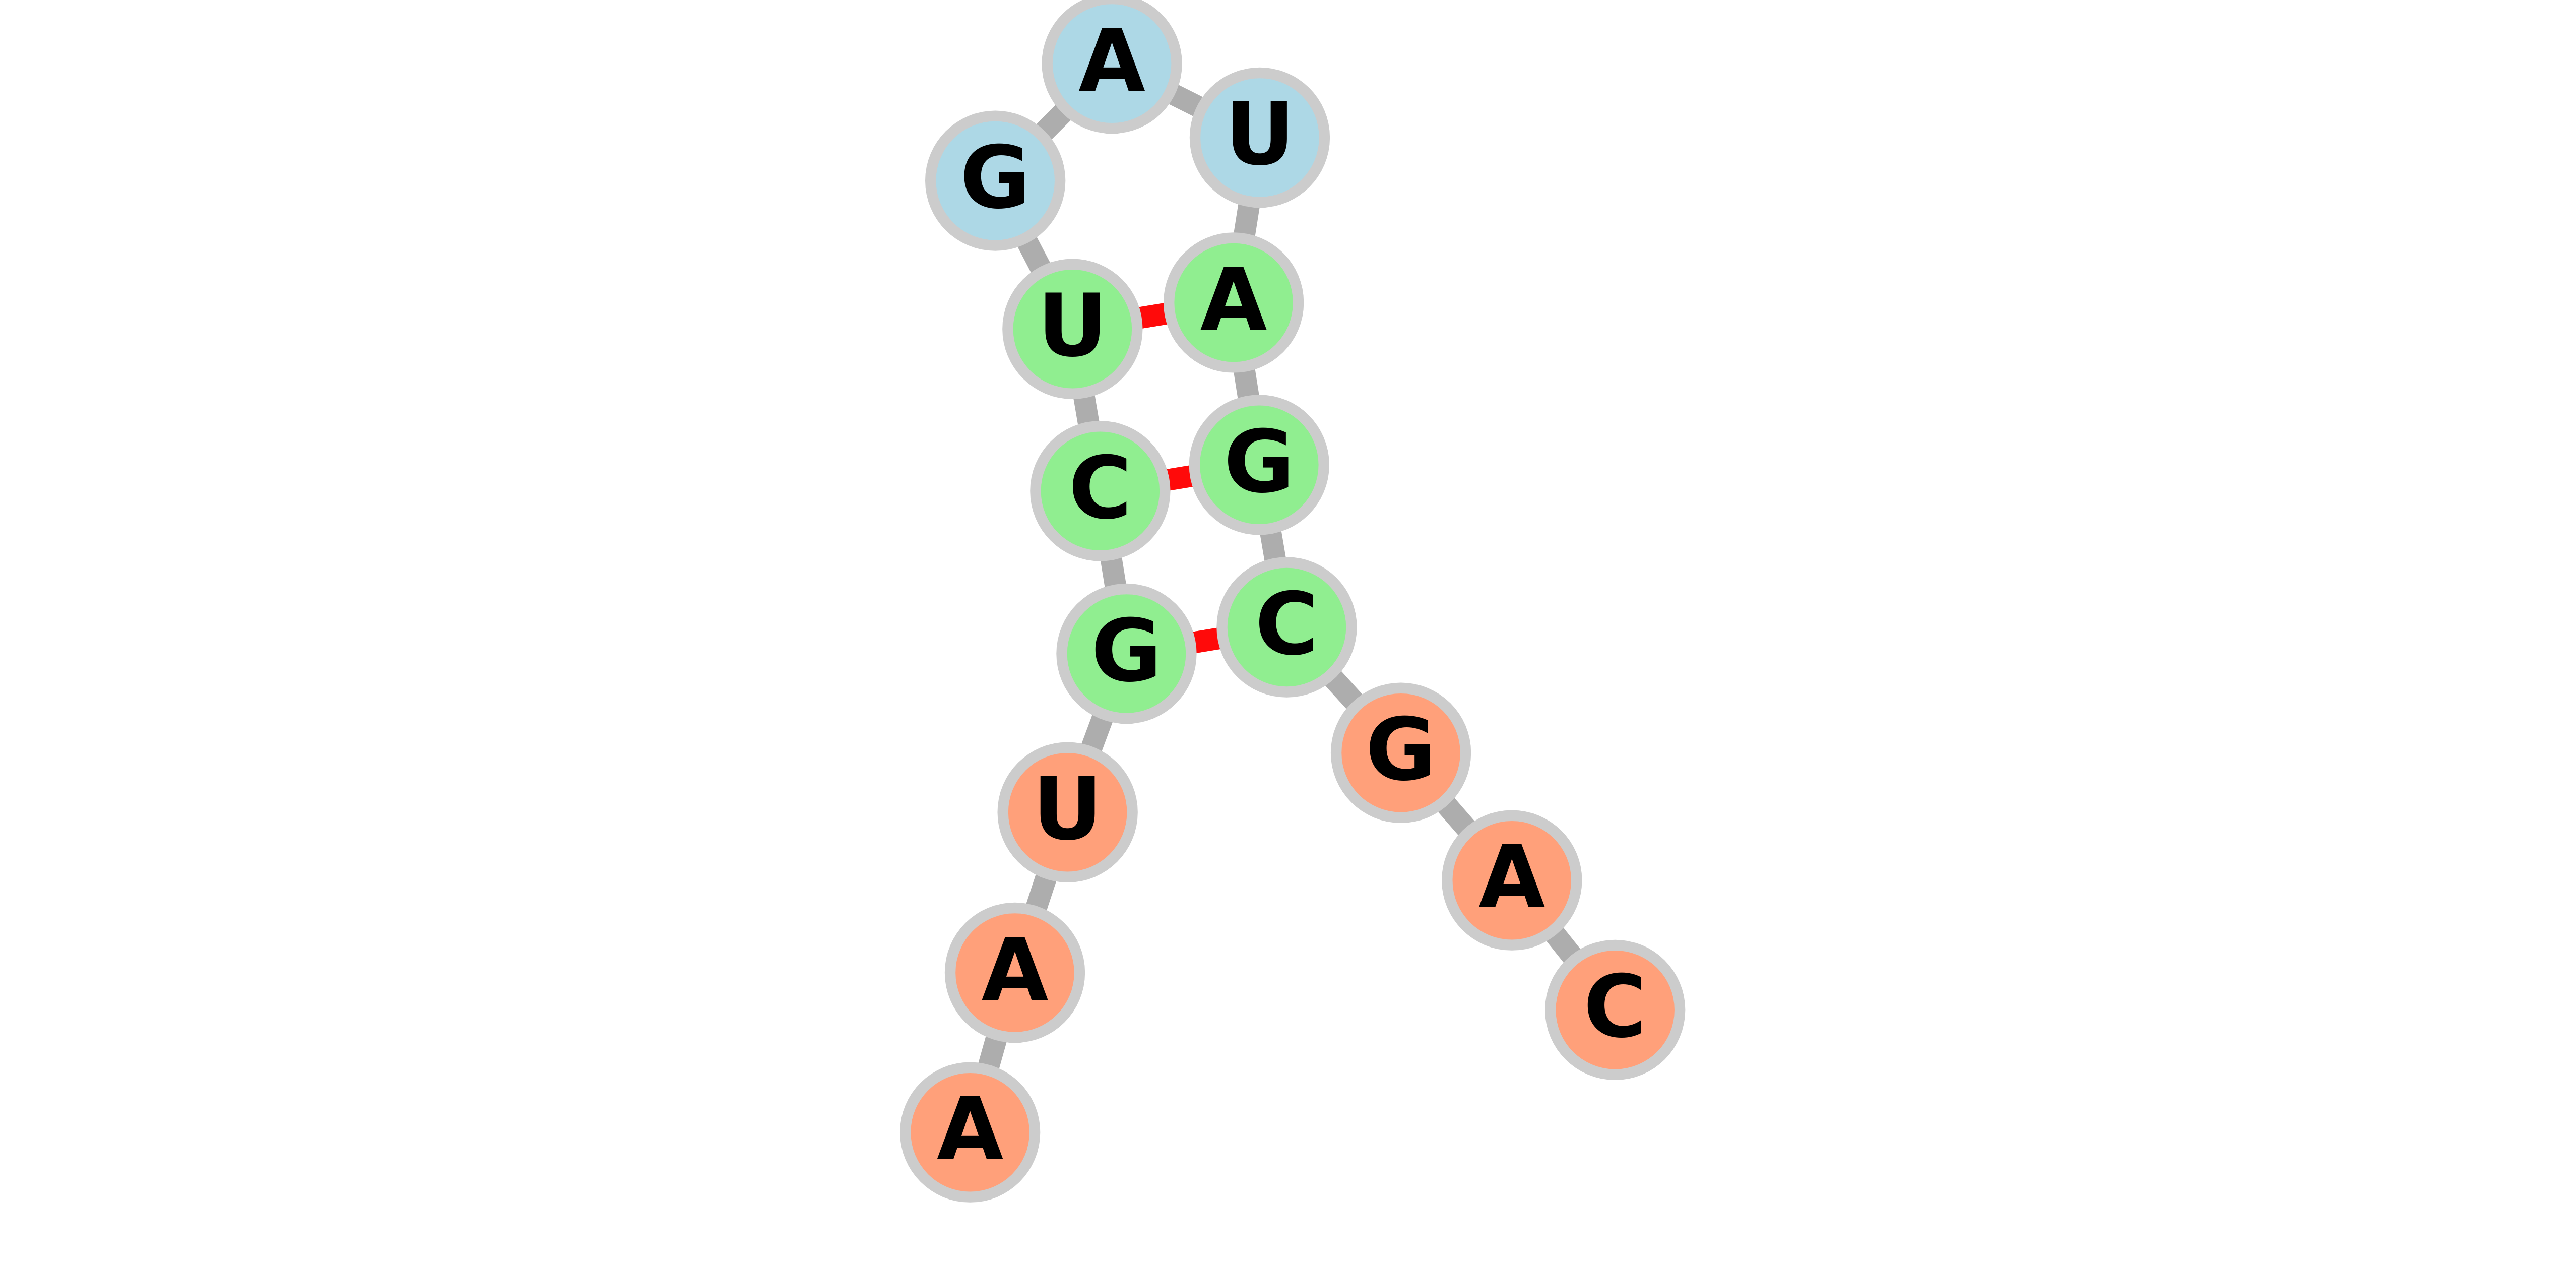
\includegraphics[width=\textwidth]{pic/intro/rnastructure.png}
		\caption{obtained using Forna \parencite{kerpedjiev_forna_2015}.
		}\label{fig:strucrepresentation:a}
	\end{subfigure}%
	\begin{subfigure}[t]{0.5\textwidth}
		\centering
		%\includegraphics[width=\textwidth]{pic/results/fig.pdf}
		\begin{minipage}[b][3cm][c]{0.5\textwidth}
			\large
			\begin{verbatim}
				...(((...)))...
				AAUGCUGAUAGCGAC
			\end{verbatim}
		\end{minipage}
		\caption{dot-bracket notation.
		}\label{fig:strucrepresentation:b}
	\end{subfigure}
	\caption[Structure Representation]{
		\begin{enumerate*}[label={(\alph*)}, font={\bfseries}]
			\item A simple RNA secondary structure and
			\item its dot-bracket notation aligned with the primary nucleotide sequence.
		\end{enumerate*}
	}\label{fig:strucrepresentation}
\end{figure}

The so-called dot-bracket notation uses dots to denote unpaired positions and matching pairs of brackets or parentheses for base pair positions (\autoref{fig:strucrepresentation:b}).

\end{document}
